\documentclass[Main]{subfiles}
\begin{document}


%NUMBERING of all subsubsection ecc (in order to better grasp the quantization procedure scheme)
\setcounter{secnumdepth}{5} % seting level of numbering (default for "report" is 3). With ''-1'' you have non number also for chapters
\renewcommand\thesubsubsection{\Alph{subsubsection}}
\renewcommand\theparagraph{\thesubsubsection.\alph{paragraph}}
\renewcommand\thesubparagraph{\theparagraph.\Roman{subparagraph}}

\chapter{Geodesic Fields}
	%mettere nell'intro una breve introduzione al problema geodetico nell'approccio standard della geometria riemmaniana
	In the context of differential geometry, \emph{geodesic curves} are a generalization of \emph{straight lines}  in the sense of self-parallel curves.\\
	%Definizione di geodetica su varietà con connessione
	Considering a differential manifold $M$ endowed with an affine connection $\nabla$ we define:
	\begin{definition}[Geodesic]
		A smooth curve $\gamma:[a,b]\rightarrow M$ such that:
		\begin{equation}
			\nabla_{\dot{\gamma}}\dot{\gamma} =0
		\end{equation}
		where $\dot{\gamma}^\mu \coloneqq \frac{d \gamma^\mu}{d t}$ is the tangent vector to the curve.
	\end{definition}
	

		In local chart the previous equation assumes the well-known expression:
		\begin{equation}\label{GeodesicEquation}
			\ddot{\gamma}^i + \Gamma^i_{\, j k} \dot{\gamma}^j \dot{\gamma}^k = 0
		\end{equation}
		where $ \Gamma^i_{\, j k}$ is the coordinate representation of the Christoffel symbols of the connection.
		Equation (\ref{GeodesicEquation}) admits a well-posed Cauchy problem.
		\begin{theorem}
			Let $M$ be a smooth manifold, $p\in M$, $v \in T_p M$. 
			Then there exist $\epsilon>0$ and precisely one geodesic
			\begin{displaymath}
				c: [0,\epsilon]\rightarrow M
			\end{displaymath}
			with $c(0) = p , \dot{c}(0) = v$.\\
			 In addition, $c$ depends smoothly on $p$ and $v$.
		\end{theorem}
		\begin{proof}
		Equation \ref{GeodesicEquation} is a system of second order ODE, and the Picard-Lindelof theorem yields the local existence and uniqueness of a solution with prescribed initial values and derivatives, and this solution depends smoothly on the data.
		\end{proof}

	\vspace{4mm}
	%Definizione metrica di geodetica su varietà riemmaniana( con connessione di levi civita)	
	In presence of a pseudo-Riemannian metric it is possible to present the geodesic %in a metric sense i.e. 
	as the curve extremizing the \emph{Energy Functional}\footnote{Remember that for arc-length parametrized curves the Energy functional coincides with the length functional.\cite[Lemma $1.4.2$ ]{Jost2005}}:
	\begin{definition}[Energy functional]
  	\begin{equation}\label{EnergyFunctional}
  		H: C^1\left(\left[a,b\right],Q\right) \rightarrow \Real \qquad
 		H(\gamma) \coloneqq \int_a^b \left\Vert \frac{d \gamma}{dt} (t)\right\Vert^2 dt
 	\end{equation}
\end{definition} 	
	Considering only the proper variations (that keep the end-point fixed), the extremum condition corresponds to equation \ref{GeodesicEquation} where $\nabla$ is the unique Levi-Civita connection (torsion-free and metric-compatible).

	\vspace{4mm}
		%Problema di Jacobi, deviazione geodetica e legame alla curvatura
	In general relativity the problem of the 
	linearization of the geodesic equation yields the Jacobi equation which takes
	%geodesic equation linearization, named \emph{Jacobi equations} takes
	 a central role. \footnote{Usually in this context takes the name of \emph{Geodesic deviation} problem\cite[pag. 46]{Wald1984} inasmuch Jacobi field describes the difference between the geodesic and an "infinitesimally close" geodesic.}
	
	\begin{definition}[Jacobi Field]
	We call a \emph{Jacobi field} along the geodesic $\gamma$ the tangent vector field over the submanifold $\gamma(t,\tau)$, determined by  a smooth one parameter family of geodesics$ \gamma_\tau$ ( with $\gamma_0=\gamma$), in respect to the$\tau$ coordinate. \textit{i.e.}:
	\begin{displaymath}
	 J = \left. \frac{\partial \gamma_\tau (t)}{\partial \tau}\right\rvert_{\tau=0}
	\end{displaymath}
	\end{definition}
	
		In local charts, a Jacobi field along the geodesic $\gamma$ is solution of a linear O.D.E.:
		\begin{equation}\label{JacobiEquationComponents}
			\big( X''\big)^\mu + R^\mu_{i \alpha \j} T^i X^\alpha T^j =0
		\end{equation}
		where:
		\begin{itemize}
			\item $\big(X'\big)^\mu \coloneqq \big( \nabla_{\dot{\gamma}(t)} X\big)^\mu$ is the covariant derivative along the curve $\gamma$.
			\item $T \equiv \dot{\gamma}(t)$ stands for the tangent vector to $\gamma$.
			\item $R^\mu_{i \alpha \j}$ are the representation in components of the Riemann curvature tensor,
		\end{itemize}

	
	
	
	
	The rest of this chapter will be devoted to discussing geodesic and Jacobi fields
	% the presentation of the approach to geodesic and Jacobi problem 
	as a physical system.


\section{Geodesic Problem as a Mechanical Systems}\label{GeodesicMechanics}
	% Da quanto detto in introduzione ha un odore molto forte il legame  dell'equazione geodetica con l'equazione del moto di un punto su una varietà e dell' funzionale lunghezza come versione con il prinicpio di minima azione
	The basic idea is very simple, to portray the geodesic curve as the natural motion of a free point particle constrained on the Pseudo-Riemannian manifold $Q$.
	
	\begin{remark}
	In terms of general relativity this problem can be instantly recognized as the derivation of the motion of free-falling particles.
	
	However, there is no lack of alternative viewpoints .
	The framework of the classical \emph{geometric mechanics} taught us to picture the "static" configurations of a constrained, complex, classical system as a point on the \emph{Configuration space}.% manifold. 
	According to that, the geodesic motion can be seen as a realization of a particular dynamics on a mechanical system with a pseudo-Riemannian configuration space\footnote{Such systems can be depicted as "geodesic" even in presence of a position-dependant potential.\cite[Cap 3.7]{Abraham1978}}.
	\end{remark}


	% Q è la varietà riemmanian in esame, eccc. vedi pag 223  e successive del fomm (direi di dare per assodato tutto il contesto di meccanica geometrica che mi sono studiato nei primi mesi della tesi ma credo non sia il caso di mettere per esteso qui, al massimo solo linkarlo

	\begin{proposition}[Geodesic Motion]
		The geodesics on the Pseudo-Riemannian manifold $(Q,g)$ are the natural motions of the ordinary Lagrangian system $(Q, L)$ where:
		\begin{equation}
			L(V_q) \coloneqq \frac{1}{2} g_q(V,V)
		\end{equation}
	\end{proposition}	
	\begin{proof}
		%	 The Euler-Lagrange equation of $L$ coincides with the geodesic equation \ref{GeodesicEquation}.
		%	 \danger.. è sul quaderno non so se metterla (ho dovuto staccare i foglio per portarmeli a lecce!) ora sono pinzati al quanderno 2
		A direct computation of the Euler-Lagrange equations:
		\begin{displaymath}
			\frac{d}{dt} \left( \frac{\partial L}{\partial V^i}\right) = \frac{\partial L}{\partial q^i}
		\end{displaymath}
		for the Lagrangian
		\begin{displaymath}
			L = \frac{1}{2} g_{i j} ( \vec{q} ) V^i V^j
		\end{displaymath}
		brings to the following equation motion:
		\begin{displaymath}
			g_{k j} \ddot{q}^j = \left(
				 \frac{1}{2} \left(
				 	\frac{\partial g_{i j}}{\partial q^k} \dot{q}^i \dot{q}^j \right)
				  - \frac{\partial g_{k j}}{\partial q^i} \dot{q}^i \dot{q}^j  \right)
		\end{displaymath}
		Multiplying for the inverse of the metric we find:
		\begin{displaymath}
			g^{l k} g_{k j } \ddot{q}^j \equiv \ddot{q}^l = \frac{1}{2} g^{l k} \left( \frac{\partial g_{i j}}{\partial q^k} - \frac{\partial g_{k j}}{\partial q^i}- \frac{\partial g_{k i}}{\partial q^j}\right) \dot{q}^i \dot{q}^j 
			= - \Gamma^l_{\, i j} \dot{q}^i \dot{q}^j
		\end{displaymath}
		where in the last equation we have recognized the expression of Christoffel symbols in term of the Riemannian metric.
	\end{proof}

%	\begin{observation}
	\begin{remark}
		The geodesic system is not simply Lagrangian but also Hamiltonian.
		This property follows from the hyperregularity\cite{Abraham1978} of $L$.
	\end{remark}
%	\end{observation}

	%Qualsiasi sistema di mqo come il precedente può essere visto come un sistema campo.
	As shown in chapter 2, every system with discrete degrees of freedom can be seen as a trivial field system.
	From that it follows the alternative characterization of geodesics as a Lagrangian field:
	\begin{corollary}[Geodesic field]
		The geodesics on the Pseudo-Riemannian manifold $(Q,g)$ can be seen as the \emph{Dynamical Configurations} of the Lagrangian field system $(E,\Lagrangian)$ where:
		\begin{itemize}
			\item $E=(Q\times\Real, \pi, \Real)$ trivial smooth bundle on the real line.
			\item $\Lagrangian[\gamma] = \frac{1}{2} g(\dot{\gamma},\dot{\gamma})(t) dt$
		\end{itemize}
	\end{corollary}
	\begin{proof}
		It is a simple application of the correspondence seen in chapter \ref{MechanicsAsAField}.
	\end{proof}
	
	From this perspective it is clear that the Energy Functional corresponds to the action of the geodesic field dynamics and equation \ref{GeodesicEquation} is nothing more than the equations of motion according to the \emph{least action principle}.

% \danger aggiungere!!!
%		\begin{figure}[h!]
%		 \centering
   	%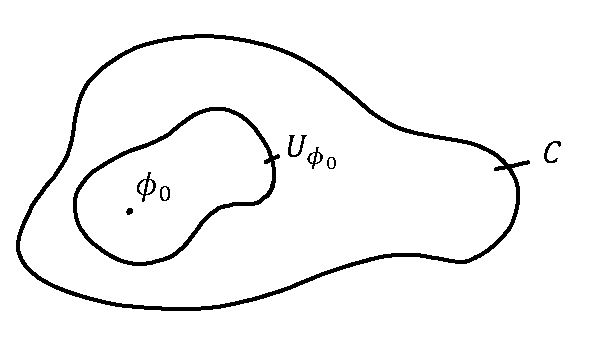
\includegraphics[width=0.5\textwidth]{Pictures/Linearization} 
   	% (credo sia la figura pagina 1 del quaderno 2)
%	 	 \caption{Impressionistic view of the geometric mechanics structure.}
%		\end{figure}		


\section{Peierls Bracket of the Geodesic field}
	The local coordinate expression for the Lagrangian density of the geodesic field is:
	\begin{equation}
		\Lagrangian\big(t,\gamma^i(t), \dot{\gamma}^i(t) \big)\coloneqq \frac{1}{2}g_{\mu,\nu}\left(\gamma^i\left(t\right)\right)\dot{\gamma}^\mu \dot{\gamma}^\nu
	\end{equation}		
	which is highly non-linear. \\
	It is explicitly is quadratic in the velocity components $\dot{\gamma}^i$ and implicitly, through $g_{\mu\nu}(\gamma^i(t))$, is non-polynomial in the %curve 
	coordinates $\gamma^i$.
	
	As show in section \ref{Section:NonLinearPeierls}, for this type of systems the calculation of the Peierls bracket can be realized only locally around a predetermined solution.
	Let us repeat the Peierls' procedure for the system under investigation.

	As a consequence of our introduction on the geodesic as a field, we can state the unperturbed dynamic as a L.P.D.O :
		\begin{equation}
			Q_\Lagrangian \big(q^\mu 	\big)= \biggr[\ddot{q}^\mu + \Gamma^\mu_{\, i j}\dot{q}^i \dot{q}^j	\biggr]
		\end{equation}
	where $\dot{q}^\mu = \frac{d}{dt}q^\mu(t)=\dot{q}^i\partial_i q^\mu$.
	
	A linear variation of $q_0^\mu +\epsilon \eta^\mu$ constructed from the coordinate representation $q_0^\mu$ of the geodesic $\gamma_0 \in \Sol$, solves the original equations of motion when
	\begin{equation}\label{GeodesicJacobation1}
		Q_\Lagrangian \big( q_0^\mu +\epsilon \eta^\mu \big) = \frac{d^2}{dt^2}\biggr( q_0^\mu +\epsilon \eta^\mu \biggr) +
		\biggr[ \Gamma^\mu_{\, i j}\big( \vec{q_0} + \epsilon \vec{\eta}\big) \biggr]\biggr(\dot{q_0}^i +\epsilon \dot{\eta}^i \biggr)\biggr(\dot{q_0}^j +\epsilon \dot{\eta}^j \biggr) = 0 \mbeq o(\epsilon)
	\end{equation}
	If we consider only the first order in the parameter $\epsilon$ we can expand the expression of the Christoffel symbols:
	\begin{displaymath}
		\biggr[ \Gamma^\mu_{\, i j}\big( \vec{q_0} + \epsilon \vec{\eta}\big) \biggr] =
		\biggr[ \Gamma^\mu_{\, i j}( \vec{q_0}) + \epsilon \eta^\alpha\big( \partial_\alpha  \Gamma^\mu_{\, i j} \big)\biggr\vert_{\vec{q_0}} + o(\epsilon) \biggr]
	\end{displaymath}	 
	
	Collecting all the terms in equation \ref{GeodesicJacobation1} up to the first order in $\epsilon$ it follows a condition on the perturbation:
	\begin{align}\label{Eq:JacobiPeierlsEquation}
	0 &= \ddot{\eta}^\mu + \eta^\alpha\big( \partial_\alpha  \Gamma^\mu_{\, i j} \big)\biggr\vert_{\vec{q_0}} \dot{q_0}^i \dot{q_0}^j  +  \Gamma^\mu_{\, i j} \big(\dot{\eta}^i \dot{q_0}^j + \dot{q_0}^i \dot{\eta}^j \big)= \nonumber \\
	&=\biggr\{ g^\mu_{\,\alpha} \frac{d^2}{dt^2} +
	 \Gamma^\mu_{\, i \alpha}(\vec{q_0})\big[2 \dot{q_0}^i \frac{d}{dt} \big] + 
\big[ \partial_\alpha \Gamma^\mu_{\, i j}(\vec{q_0}) \dot{q_0}^i \dot{q_0}^j  \big] \biggr\} \eta^\alpha	= P^\mu_{\: \alpha} \eta^\alpha
	\end{align}		
	where $ P^\mu_{\: \alpha}$ is a linear partial differential operator acting on the \emph{variations} \textit{,i.e.,} the components of a field along the geodesic $\gamma_0$.\\
	As showed in section \ref{Section:NonLinearPeierls}, equating the linearized dynamics operator with the term $-\left(Q_\chi(\gamma_0)\right)(x)$ 	(see equation \ref{PeierlJacobiEqNonLin}) leads to the inhomogeneous \emph{Jacobi operator} from which all the standard construction of the brackets Peierls follows.

	
	\begin{proposition}
		The differential equation $$P^\mu_{\: \alpha} \eta^\alpha=0$$ corresponding to the l.p.d.o $P$ defined in equation \ref{GeodesicJacobation1} corresponds to equation \ref{JacobiEquationComponents} defining  the \emph{Jacobi fields} along the geodesic $\gamma_0$.
	\end{proposition}
	\begin{proof}
		For convenience, we adopt the following notation:
		\begin{align*}
		&\eta^\mu \partial_\mu \coloneqq X \equiv X^\mu \partial_\mu \\
		&\dot{q_0}^i \partial_i \equiv \dot{\gamma_0} \coloneqq T \equiv T^i \partial_i
		\end{align*}
		We have to show that the equation just found:
		\begin{equation}\label{JacobiEqI}
			\ddot{X}^\mu + X^\alpha\left(\partial_\alpha\Gamma^{\mu}_{\, i j}\right)T^i T^j + \Gamma^\mu_{\, \alpha j}\left(2 T^j \dot{X}^\alpha \right) = 0
		\end{equation}
		where $\dot{X}^\mu = \frac{d}{dt}X^\mu= T^i \partial_i X^\mu$,
		corresponds to the equation defying the Jacobi field:
		\begin{equation}\label{JacobiEqII}
			\left(X'' \right)^\mu + R^\mu_{\, i \alpha j}T^i X^\alpha T^j = 0
		\end{equation}
		where $\left(X')\right)^\mu \coloneqq \left(D_t X \right)^\mu$ and $D_t = T^i \nabla_i$ is the covariant derivative along the curve.\\
		Since:
		\begin{align}\label{JacobiEqDerivative}
			X'' &= D_t D_t X = D_t \left( \partial_\mu \left( \dot{X}^\mu + \Gamma^\mu_{\, i \alpha} T^i X^\alpha \right)\right) \nonumber \\
			&=\left( \ddot{X}^\mu + \frac{d}{dt}\left( \Gamma^\mu_{\, j \alpha} T^j X^\alpha \right) + \Gamma^\mu_{\, j \nu}T^j \dot{X}^\nu + T^j \Gamma^\mu_{\, j \nu} \Gamma^\nu_{\, i \alpha} T^i X^\alpha \right)\partial_\mu
		\end{align}
		We can write equation \ref{JacobiEqI} in term of the covariant derivative as:
		\begin{align*}
			\left(X'' \right)^\mu &=
			- \left(
			X^\alpha\left(\partial_\alpha\Gamma^{\mu}_{\, i j}\right)T^i T^j + \Gamma^\mu_{\, \alpha i}\left(2 T^i \dot{X}^\alpha \right)
			- \frac{d}{dt}\left( \Gamma^\mu_{i \alpha} T^i X^\alpha \right) - T^j \Gamma^\mu_{\, j s} \Gamma^s_{\, i \alpha} T^i X^\alpha
			\right) =\\
			&=			
			-\left(
			X^\alpha\left(\partial_\alpha\Gamma^{\mu}_{\, i j}\right)T^i T^j - \dot{\Gamma}^\mu_{i \alpha} T^i X^\alpha
			- \Gamma^\mu_{i \alpha} \dot{T}^i X^\alpha  - T^j \Gamma^\mu_{\, j s} \Gamma^s_{\, i \alpha} T^i X^\alpha				
			\right)
		\end{align*}
		remembering that the geodesic condition is still to be met:
		\begin{displaymath}
			\dot{T}^i = - \Gamma^I_{\, j k} T^j T^k
		\end{displaymath}
		we can conclude that:
		\begin{align*}
			\left(X'' \right)^\mu &=
			- \left(
			  X^\alpha\left( \partial_\alpha\Gamma^\mu_{\, i j}\right)T^i T^j
			- T^j \left( \partial_j \Gamma^\mu_{\, i \alpha}\right) T^i X^\alpha
			+X^\alpha \Gamma^\mu_{\, \alpha s} \Gamma^s_{\, i j}T^i T^j 
			- T^j \Gamma^\mu_{\, j s} \Gamma^s_{\, i \alpha} T^i X^\alpha
			\right) =\\
			&=	-\left( R^\mu_{\, i \alpha j}T^i X^\alpha T^j\right)		
		\end{align*}
	\end{proof}
	
	

	
	

\subsection{Example: Geodesic field on FRW space-time.}
\ifToninus
	\begin{Warning}
	% qui i conti li devo ancora fare, 
	l'idea è che per scelta di metrica e geodetica semplici le equazioni di jacobi possono essere disaccoppiate a dare 4 ode di cui in linea di principio posso calcolare la funzione di green	

	\vspace{2mm}
	Per Ripasso di FRW: \url{http://universeinproblems.com/index.php/Friedman-Lemaitre-Robertson-Walker_(FLRW)_metric#Problem_1:_expanding_baloon}

	\vspace{2mm}
	L'esempio deve articolarsi così:
		\begin{enumerate}
			\item Introdurre la Metrica FRW come fa CD (ricordare che è GH)
			\item Calcolo Cristoffel (uso Mathematica)
			\item Equazione Geodetica
			\item Calcolo R
			\item Do espressione in coordinate per il campo di Jacobi
			\item Verifico che trovo 4 equazioni Disaccoppiate (credo che sarà necessario mettersi nelle coordinate che dice Wiki)
			\item calcolo le 2 soluzioni omogenee per ogni componente
			\item ricordare cos'è l'operatore di green in generale, se l'op è diagonale ricordare come si semplifica (cioè ho 4 op di green per ogni ode), ricordare cos'è l'op di green per una ode (cioè operatore  a nucleo integrale, il nucleo è detto 
			\item Criterio per il calcolo delle green per delle ode lineari di secondo ordine
			\item realizzo il calcolo per ogni componente di jacobi
			\item realizzo l'op di green (dovrebbe dipendere dalla geodetica da cui sono partito ) è dico come va inserito per ottenere il disturbo
			\item limitandosi al caso di densità lagrangiane lineari trovo il disturbo e le peierls
		\end{enumerate}
	\end{Warning}
\fi	
	Let us compute the Peierls' bracket for the single special case of geodesic motion on Friedmann–Lemaître–Robertson–Walker spacetimes (FRW).
	
	We recall that the FRW spacetimes are homogeneous and isotropic solutions of Einstein’s equations.
	These manifold are endowed with a line element of the form:
	\begin{equation}
		ds^2 = -dt^2 + a^2(t) \left( \frac{dr^2}{1-k r^2} + r^2 d\theta^2 + sin^2(\theta) d\phi^2\right)
	\end{equation}
		where $0 < a(t) \in C^\infty	(\Real)$ is said \emph{scale factor} and $k$ is a constant normalizable to $\pm 1$ or $0$.
		The assumptions of homogeneity and isotropy alone determine the spacetime metric up to the three discrete possibilities of spatial geometry.
		This spacetime is topological equivalent (homeomorphic) to $\Real \times \Sigma$ where $\Sigma$ is a 3D manifolds which depends on the value of $k$:
		\begin{center}\begin{tabular}{l l}
			$k = 1$ & $\Sigma \simeq S^3$ (3-sphere)\\
			$k = 0$ & $\Sigma \simeq \Real^3$ (three-dimensional Euclidean space)\\
			$k = -1$ & $\Sigma \simeq H^3$ ( three-dimensional hyperboloid)\\		
		\end{tabular}\end{center}
		\vspace{2mm}
		
		For the sake of simplicity let reduce ourselves to the case of \emph{flat} spatial geometry, \\textit{i.e.}:
		\begin{displaymath}
			ds^2 = -dt^2 + a^2(t) \left( dx^2 + dy^2 + dz^2\right) = g_{\mu \nu} dx^\mu dx^\nu
		\end{displaymath}
		in the \emph{cosmological} reference frame.
\ifToninus
	\begin{Warning}
		Una possibile giustificazione a questa tesi è : evidenze sperimentali in ambito cosmologico suggeriscono che $k=0$
	\end{Warning}
\fi


		In order to express the geodesic equations we have to compute the Christoffels symbols. According to the basic definition:
		\begin{displaymath}
			\Gamma^\lambda_{\, \mu \nu} = \frac{1}{2} g^{\lambda \sigma } \left( \partial_\mu g_{\sigma \nu} + \partial_\nu g_{\mu \sigma} - \partial_{\sigma}g_{\mu \nu} \right)
		\end{displaymath}
		we find that the non-vanishing components of $\Gamma^\lambda_{\, \mu \nu}$ are merely:
			\begin{eqnarray}
				\Gamma^0_{\, i i} &= a \dot{a} \\
				\Gamma^i_{\, i 0} &= \Gamma^i_{\, 0 i} = \dfrac{\dot{a}}{a}
			\end{eqnarray}
			where we have used the usual convention to express with latin indices the spatial cordinate, with $0$ the time coordinate and with greek indices all the spacetimes coordinates.
			
			In the cosmological coordinate chart the geodesic equations are:
			\begin{eqnarray}
				\frac{d^2}{d \tau^2} \gamma^0 &= - a \dot{a} \left( \frac{d}{d \tau} \gamma^i \frac{d}{d \tau}\gamma_i \right) \label{FRWGeo1}\\
				\frac{d^2}{d \tau^2} \gamma^i &= - 2 \dfrac{\dot{a}}{a} \left( \frac{d}{d \tau} \gamma^0 \frac{d}{d \tau}\gamma^i \right) 		\label{FRWGeo2}	
			\end{eqnarray}
			
			Jacobi fields are dependant from the choice of a base geodesic. 
			Let us consider the a simple time-like geodesic, namely the \emph{cosmological} free-falling observer:
			\begin{displaymath}
				\gamma^\mu (t) = \begin{bmatrix}  a_0 + m t \\  a_1 \\ a_2 \\ a_3  \end{bmatrix}
				\qquad
				T^\mu=\frac{d}{d t}\gamma^\mu(t)= \begin{bmatrix}  m \\  0 \\ 0 \\ 0  \end{bmatrix}
			\end{displaymath}
\ifToninus
	\begin{Warning}
		Sul quaderno ho scritto un po' di più rifacendomi al discorso visto su wiki Jacobi Fields.
	\end{Warning}
\fi
			Remembering the definition of Riemannian curvature:
			\begin{displaymath}
				{R^\sigma}_{\mu\nu\kappa} =
				  {\partial{\Gamma^\sigma}_{\mu\nu} \over \partial x^\kappa} -
				  {\partial{\Gamma^\sigma}_{\mu\kappa} \over \partial x^\nu} +
				  {\Gamma^\lambda}_{\mu\nu}{\Gamma^\sigma}_{\kappa\lambda} -
				  {\Gamma^\lambda}_{\mu\kappa}{\Gamma^\sigma}_{\nu\lambda}		
			\end{displaymath}			 
			we find by direct computation  that the non-null components of the Riemann curvature tensor are:
			\begin{equation}
				R^0_{\: i 0 i}= - R^{0}_{\: i i 0}= a \ddot{a} \qquad
				R^i_{\: 0 0 i}=-R^i_{\: 0 i 0}=	\dfrac{\ddot{a}}{a}\qquad
				R^i_{\: j i j} = - R^i_{\: j j i} = \dot{a}^2				
			\end{equation}
			Since we have parametrized the curve by coordinate $x^0 = t$ the covariant derivative in Eq. \ref{JacobiEquationComponents}  corresponds to an ordinary derivative, then a Jacobi $X^\mu(t)$ along the time-like geodesic $\gamma(t)$ satisfies the following uncoupled homogeneous equations:
			\begin{eqnarray}
				\frac{d^2}{d t^2} X^0  &=& 0 \label{FRWJacobi1}\\
				\frac{d^2}{d t^2} X^i &= &- m^2 R^{\mu}_{\: 0 \nu 0} X^\nu = \left( m^2 \frac{\ddot{a}}{a}\right) X^i 	\label{FRWJacobi2}	
			\end{eqnarray}			
			\vspace{2mm}
			
			Regarding this problem as a field system, we can say that the operator $P$ ruling the dynamics is diagonal:
			\begin{displaymath}
				P X =
				 \begin{bmatrix}  
				 \left(\frac{d}{dt}\right)^2 & 0 \\
				 0 & \IdOp \left( \left(\frac{d}{dt}\right)^2 - m^2 \frac{\ddot{a}}{a} \right)
				 \end{bmatrix}
				 \begin{bmatrix} X^0 \\ X^i  \end{bmatrix}
				 = 0
			\end{displaymath}
			
			The main difficulty to face in the explicit Peierls brackets construction is the computation of the Green operator of $P$.
			In this case we can say with certainty that both Green operators are diagonal:
			\begin{displaymath}
				G^\pm =
				 \begin{bmatrix}  
				 G\pm_0 & 0 \\
				 0 & G^\pm_i
				 \end{bmatrix}
			\end{displaymath}		
			where $G^\pm_0$ and $G^\pm_i$ are the Green operators of the only two ODE involved:
			\begin{displaymath}
				P_0 = \left(\frac{d}{dt}\right)^2 \qquad P_i=\left( \left(\frac{d}{dt}\right)^2 - m^2 \frac{\ddot{a}}{a} \right)
			\end{displaymath}
			Namely these operators are the Hilbert–Schmidt integral operators:
			\begin{displaymath}
				G^\pm_\mu f = \int_\Real G^\pm_\mu( x \vert \xi ) f(\xi) d\xi
			\end{displaymath}
			where the kernel function $G^\pm( x \vert \xi ) $ it is known as \emph{Green function} and satisfies the fundamental distributional equation:
			\begin{equation}\label{Eq:FoundamentalEquation}
				P_\mu G^\pm_\mu( x | \xi) = \delta( x - \xi)
			\end{equation}
\ifToninus
	\begin{remark}
		\danger .. L'utilizzo principale di questi oggetti è per il calcolo della soluzione particolare delle ODE inomogenee.
	\end{remark}
\fi			
			In the specific case of second order ODE the general Green function  - solution of equation \ref{Eq:FoundamentalEquation} - can be explicitly computed as a linear combination of two linearly independent solutions $y_1$ and $y_2$ of the homogeneous problem:
			\begin{equation}
			\begin{cases}
                        G( x \vert \xi) = \theta( x - \xi) \left(d_1 y_1(t) + d_2 y_2(t) \right) + \theta( x - \xi) \left(c_1 y_1(t) + c_2 y_2(t) \right) \\
						y_1(\xi) (c_1-d_1) + y_2(\xi) ( c_2 - d_2) = 0 \\
						\dot{y}_1(\xi) (c_1-d_1) + \dot{y}_2(\xi) ( c_2 - d_2) = -1 \\
            \end{cases}
			\end{equation}
			where the two undetermined parameters depend on the eventual boundary conditions.
\ifToninus
	\begin{Warning}
		Sarebbe stato carino fare un'appendice sul metodo del calcolo delle green per le ode componendo due soluzioni di omogenea \cite{Tornberg}.
	\end{Warning}
\fi		
			(For a quick reference see for example \cite{Tornberg}.)
			
			 Eq. \ref{FRWJacobi1} is a linear autonomous ordinary differential equation, the advaced and retarded Green functions can be promptly computed:
			\begin{eqnarray*}
				G^+_0(t \vert \xi) = \theta(t-\xi) \left(a +b t \right) \\
				G^-_0( t \vert \xi) = \theta(\xi -t) \left( a +b t + \xi -t\right)
			\end{eqnarray*}

			In other hand, since coefficient $m^2 \frac{\ddot{a}(t)}{a(t)}$ it is generally time dependant,  Eq. \ref{FRWJacobi2} it's non-autonomous and do not exists an analytical expression of its general solution.
\ifToninus
	\begin{Warning}	
		Anche un'appendice sul calcolo delle green sfruttando lo sviluppo di Dyson e quello di Magnus ( Partendo come spunto dall'articolo \cite{Dappiaggi2014}) non sarebbe stata male. ma è venuto il tempo di concludere.
	\end{Warning}
\fi	
			However it is possible to express the corresponding Green function as a convergent Dyson expansion\cite{Dappiaggi2014}.
			The idea is to consider the non-autonomous term $V(t) = -m^2 \frac{\ddot{a}(t)}{a(t)}$ as if it were a perturbing potential.\\
			Remembering that $G^\pm_0 (t \vert \xi)$ is the Green function of operator \ifToninus$P_{0}=\left(\frac{d}{dt}\right)^2$\else$P_0$\fi, which can be seen as the time-independent part of differential operator \ifToninus$P_{i i}=\left( \left(\frac{d}{dt}\right)^2 - m^2 \frac{\ddot{a}}{a} \right)$\else$P_i$\fi, we can express the Green function of $P_{i}$ as follow:
			
			\begin{align*}
				G^+_i ( \tau \vert \tau' ) = G^+_0( \tau \vert \tau' ) + \sum_{n=1}^\infty (-)^n 
				\int_{-\infty}^\tau dt_1 \cdots \int_{-\infty}^{t_{n-1}} dt_{n-1} 
				& \times	  G^+_0(\tau \vert t_1) G^+_0(t_1\vert t_2) \cdots G^+_0(t_{n-1} \vert t_n) \times \\
				& \times  V(t_1) V(t_2) \cdots V(t_n) \times \\
				& \times  G^+_0 (t_n \vert \tau' ) \\
			\end{align*}		
			similarly $G^-_i$  can be obtained considering the anticipated Green function $G^-_0$ and integrating from $t$ to $+\infty$.
			
			\vspace{2mm}
		Anyway all this machinery it is not necessary in the special case of where \emph{De Sitter} spacetimes where $ a(t) = exp(H t)$ and the coefficient $\ddot{a}/a$ is a positive constant.  \cite{Wald1984}\\
		In this case the general solutions are simply:
		\begin{displaymath}
		 y(t) = c_1 e^{m t \sqrt{\ddot{a}/a}} + c_2 e^{-m t \sqrt{\ddot{a}/a}}
		\end{displaymath}
		and the Green functions can be expressed as follows:
			\begin{eqnarray*}
				G^+_i(t \vert \xi) &=& \theta( x - \xi) \left(a e^{m t \sqrt{\ddot{a}/a}} + b e^{-m t \sqrt{\ddot{a}/a}}\right) \\
				G^-_i( t \vert \xi) &=& \theta(\xi -t) \left( 
				\left(a-\frac{e^{-\xi m \sqrt{\ddot{a}/a}}}{2 m \sqrt{\ddot{a}/a}} \right) e^{m t \sqrt{\ddot{a}/a}}+
				\left(b +\frac{e^{\xi m \sqrt{\ddot{a}/a}}}{2 m \sqrt{\ddot{a}/a}} \right) e^{m t \sqrt{\ddot{a}/a}}			
				\right)
			\end{eqnarray*}

			Combing all these results we're able to give an explicit expression of the Peierls symplectic form $\tau$- as defined in Eq. 	\ref{Def:SymplecticTau}- for the De Sitter spacetime.
			For any pair $(X, Y)$ of compactly supported fields over $\gamma(t)$ we have:
			\begin{align*}
			\{X ,Y \} =&\int \left\langle X, \left(\GreenAdv - \GreenRet \right)Y \right\rangle dt =	\\
			=&
			\int_\Real dt  
				 \begin{bmatrix}  
					 X^0(t) & \vec{X}(t) \\
				 \end{bmatrix}
				 \begin{bmatrix}  
				 	-1 & 0 \\
				 	0 & a^2(t)\IdOp
				 \end{bmatrix}			
				 \begin{bmatrix}  
				 	(G^-_0 - G^+_0) & 0 \\
				 	0 & (G^-_i - G^+_i)
				 \end{bmatrix}	
				 \begin{bmatrix}  
				 	Y^0(t) \\ \vec{Y}(t)
				 \end{bmatrix}	
				 = \\
			=&
				\int_\Real dt  \left(
					-X^0(t) (G^-_0 - G^+_0)Y^0(t)+
					a^2(t)\vec{X} \cdot (G^-_i- G^+_i)\vec{Y}(t)
				\right) = \\
			=&
				\int_\Real dt 				\int_\Real d\xi \left(
					-X^0(t)Y^0(\xi)\left(
					\theta(\xi -t) \left( a +b t + \xi -t\right) -  \theta(t-\xi) \left(a +b t \right)
					\right) \right. +\\
			&+
					\int_\Real dt 				\int_\Real d\xi a^2(t) \left(
					\vec{X}(t) \cdot \vec{Y}(\xi)
					\left(
					 \theta(\xi -t) \left( 
				\left(a-\frac{e^{-\xi m \sqrt{\ddot{a}/a}}}{2 m \sqrt{\ddot{a}/a}} \right) e^{m t \sqrt{\ddot{a}/a}}+
				\left(b +\frac{e^{\xi m \sqrt{\ddot{a}/a}}}{2 m \sqrt{\ddot{a}/a}} \right) e^{m t \sqrt{\ddot{a}/a}}			
				\right)\right)
					\right)+ \\
			&-
					\int_\Real dt 				\int_\Real d\xi a^2(t) \left( 
					\vec{X}(t)\cdot \vec{Y}(\xi)
						 \left( 
							\theta( x - \xi) \left(a e^{m t \sqrt{\ddot{a}/a}} + b e^{-m t \sqrt{\ddot{a}/a}}\right)
						\right)
					\right)
			\end{align*}						

			
		

\section{Algebraic quantization of the Geodesic Field}
	The algebraic quantization scheme applies only to %linear field systems.
	systems of linear fields.
	Since equation\ref{GeodesicEquation} is highly non linear,  it is not the geodesic system that can actually be quantized but rather its linearization, the Jacobi field along a fixed geodesic $\gamma_0$.
	
		\subsubsection{Classical Framework}
			The basic idea is that, chosen a geodesic $\gamma_0$, the kinematical configurations of the Jacobi fields are tangent fields along the fixed curves.
			\paragraph{Kinematics}	
			The configuration bundle $E$ corresponds to the \emph{Pull-back bundle} $\gamma_0^*(TQ)$ of the tangent bundle along the geodesic $\gamma_0$.
			Then:
			\begin{itemize}
				\item $E$ is a vector bundle over $\Real$.
				\item The base manifold $\Real$ can be considered as a degenerate globally hyperbolic spacetime, $\CauchyClass(\Real) = \Real$.
				\item the fibers are $E_p \coloneqq T_{\gamma_0(p)}Q$
				\item $\Conf = \Gamma^\infty(E) = \mathfrak{X}(\gamma_0)$ is constituted by vector fields along the curve $\gamma_0$.
			\end{itemize}
			
			\paragraph{Dynamics}
				The coordinate representation of the motion equation is:
				\begin{displaymath}
					\left( P X \right)^\mu = (X'')^\mu + R^\mu_{\, i \alpha j } T^i T^j X^\alpha
				\end{displaymath}
				where $X\in \Conf$ and $T^i = \dot{\gamma_0}^i$.
				According to equation \ref{Eq:NormallyHyperbolicRepresentation} this operator falls exactly in the class of \emph{normally hyperbolic} operators hence it is quantizable both by  means of Peierls procedure and by means of initial data.
		
		\subsection{PreQuantum Framework}
		\subsubsection{Peierls approach}
			\paragraph{Pairing}
				%The choice of the inner product on this configuration bundle is rather obvious.
				Since $Q$ is a Riemannian manifold and $\Conf$ is composed by tangent vector fields, it is straightforward to choose as inner product on the configuration bundle $E$ the metric function defined on $Q$:
				\begin{equation}
					\left\langle X,Y \right\rangle_t \coloneqq g\left( X\left(\gamma_0(t) \right),Y\left(\gamma_0(t) \right)\right)
					\qquad \forall X,Y \in E_t
				\end{equation}
				
				It follows slavishly the definition of a pairing:
				\begin{equation}
					\left( X, Y \right) = \int_\Real \left\langle X,Y \right\rangle_t dt
				\end{equation}
				well-defined for every pair $X,Y \in \Conf$ such that $\supp(X) \cap \supp(Y)$ is compact.
				
				The operator $P$ ruling the dynamics is formally self-adjoint:
				\begin{align*}
				 ( Y, PX) &= \int Y_\mu PX^\mu dt= 
				 \int\left( Y_\mu \ddot{X}^\mu + Y_\mu R^\mu_{\, i \alpha j}T^i T^j X^\alpha \right)dt = \\
 				 &= \int\left( \ddot{Y}_\mu X^\mu + X_\mu R^\mu_{\, i \alpha j}T^i T^j Y^\alpha \right)dt =
				 \int P Y_\mu X^\mu dt=( PY, X) 				 				 
				\end{align*}
				where we have integrated by parts twice (the boundary value being null since the integrand is compactly supported) and we have exploited the curvature tensor identity:
				\begin{equation}\label{Eq:CurvatureSimmetry}
					\langle R(X,T)T,Y \rangle = \langle R(Y,T)T,X \rangle
				\end{equation}

			\paragraph{Classical Observables}
				Replicating what has been done in the general case, 
				we construct the \emph{pre-observables} as the functionals $F_f:\Conf \rightarrow \Real$ for all $f \in \Gamma_0(E)$ compactly supported fields along the geodesic $\gamma_0$:
				\begin{equation}
					F_f(X) = \int_\Real <X, f>_t dt \qquad \forall X \in \Conf
				%	F_f(X) = \int_{\dom(\gamma_0)} <X, f>_t dt \qquad \forall X \in \Conf
				\end{equation}
				The space of classical observables is then obtained through the usual quotient:
				\begin{displaymath}
					\Obs \simeq \frac{\Gamma_0}{P \Gamma_0}
				\end{displaymath}
				The observables functionals are the maps:
				\begin{displaymath}
				 F_{[f]}(X) = F_f (X) \qquad \forall X \in \Sol
				\end{displaymath}
				where $f$ is a representative of the equivalence class $[f]\in \Obs$.
			
			\paragraph{Symplectic Structure}
				The geodesic motion is a particular case of a system with finite degrees of freedom, thus the Peierls brackets between two Lagrangian functionals $\chi, \omega$ around a geodesic $\gamma_0$ tested on a function $f \in C_0^\infty(\Real)$ are given by \ref{EspressionePeierlsCampiCurve}.
				Restricting the definition to the simplest Lagrangian functionals constructible from the classical observables:
				\begin{displaymath}
					\chi [\phi] \coloneqq (\chi, \phi) \qquad \chi \in \Obs,\, \phi \in \Sol
				\end{displaymath}
				corresponding to Lagrangian densities in the form:
				\begin{displaymath}
					\chi ( \vec{q}i, \dot{\vec{q}}) \coloneqq < \chi, \vec{q}> = \chi^i q_i
				\end{displaymath}
				such that $ Q_\chi \gamma_0^i = \chi^i$, the Peierls brackets expression reduces to
				\begin{displaymath}
					\left\lbrace\chi , \omega \right\rbrace (\gamma_0) [f] = \int f(t) \left\langle\chi, \left(\GreenAdv - \GreenRet \right)\omega \right\rangle dt
				\end{displaymath}
				The test-function $f$ can be neglected for regular distributions.
%				For regular distribution can be neglected the test-function $f$.

				\vspace{3.5mm}
				We conclude that,according to the Peierls' procedure,  the classical symplectic space is the pair $(\Obs, \tau)$ where:
				\begin{displaymath}
					\tau( [\chi], [\omega]) = \{\chi , \omega \} =\int \left\langle\chi, \left(\GreenAdv - \GreenRet \right)\omega \right\rangle dt = ( \chi, E \omega) \qquad \forall \chi,\omega \in \Gamma_0(E)
				\end{displaymath}
				
				
		\subsubsection{Initial data Approach}
			\paragraph{Classical Phase Space}
				The base manifold for the configuration bundle under examination is the real line $\Real$ that can be seen as a degenerate globally hyperbolic spacetime.
				Thus each point $p\in \Real$ is a Cauchy surfaces and no further support condition can be imposed.\\
				Considering that the operator $P$ is of second order, we have:
				\begin{displaymath}
					\Phase(p) \equiv \Data(p) = \Gamma^\infty(p) \times \Gamma^\infty(p) =
					T_{\gamma_0(p)}Q \times T_{\gamma_0(p)}Q
				\end{displaymath}
				and
				\begin{displaymath}
					\Phase \simeq \Sol
				\end{displaymath}
				using the map which yields the unique solution starting from an initial data.
				
			\paragraph{Symplectic Structure on the Phase Space}		
				The general definition \ref{Def:InitialDataSymplecticForm} of the symplectic form on the classical phase space reduces to:
				\begin{displaymath}
					\Omega: \Phase(p) \times \Phase(p) \rightarrow \Complex \qquad : \qquad 					
					\Omega \biggr\{ [V_0,V_1] , [W_0, W_1] \biggr\} = g(V_1,W_0)  - g( V_0, W_1) 
				\end{displaymath}
				where $g$ is the inner product on $Q$.
				\\
				This formula can be transferred to the space of solutions:
				\begin{displaymath}
					\sigma_p: \Sol \times \Sol \rightarrow \Complex \qquad : \qquad 					
					\sigma_p \biggr\{X, Y  \biggr\} = \Omega \biggr\{ [Y(t), D_t Y(t)] , [X(t), D_t X(t)] \biggr\}
				\end{displaymath}
				\vspace{3mm}
				Mimicking what has been done in example \ref{Ex:IndipendentPhaseSpace} for the scalar field, the independence of the phase space construction from the particular choice of $p \in \Real$ can be proved.\\
				Taken $X,Y \in \Sol$ two Jacobi fields on $\gamma_0(t)$, a scalar field over $\Real$ can be defined:
				\begin{displaymath}
					J(t) \coloneqq \Omega \biggr\{ [Y(t), D_t Y(t)] , [X(t), D_t X(t)] \biggr\}
					= X^\alpha(t) g_{\alpha \beta} D_t Y^\beta(t) - 
					Y^\alpha(t) g_{\alpha \beta} D_t X^\beta(t) 					
				\end{displaymath}
				where $D_t = T^\mu \nabla_\mu$ as usual.
				This is clearly a conserved current:
				\begin{eqnarray}
					D_t J =& (D_t X)^\alpha g_{\alpha \beta} (D_t Y)^\beta - (D_t Y)^\alpha g_{\alpha \beta} (D_t X)^\alpha + X^\alpha g_{\alpha \beta} D_t D_t Y^\beta - Y^\alpha g_{\alpha \beta} D_t D_t X^\beta = \nonumber \\
					=& X^\alpha g_{\alpha \beta} PY^\beta - Y^\alpha g_{\alpha \beta} PX^\beta - X_\beta R^\beta _{\, i \alpha j}T^i Y^\alpha T^j +Y_\beta R^\beta _{\, i \alpha j}T^i X^\alpha T^j  = 0
				\end{eqnarray}
				exploiting the conditions $\nabla_\mu g_{\alpha \beta}=0$, $PX=PY=0$ and equation \ref{Eq:CurvatureSimmetry}.\\
				Hence:
				\begin{displaymath}
				\int_p^{p'} D_t J = J(p) - J(p') = 0
				\end{displaymath}
			In others words:
			\begin{displaymath}
				\sigma_\Sigma (X, Y) = \sigma_{\Sigma'} (X, Y) 
				\qquad \forall X, Y \in \Sol \; \forall \Sigma, \Sigma' \in \CauchyClass(M)= \Real
			\end{displaymath}
			
				\vspace{3.5mm}
				In conclusion, according to the initial data procedure,  the classical symplectic space is the pair $(\Sol, \sigma)$ such that:
				\begin{displaymath}
					\sigma( X, Y) = X_\mu(\Sigma) \left( D_t Y (\Sigma)\right)^\nu - \left(D_t X(\Sigma)\right)_\mu Y^\nu(\Sigma) \qquad \forall X,Y \in \Sol
				\end{displaymath}
				where $\Sigma$ is an arbitrary point in $\Real$.

	\subsection{Comparisons}
		The two procedures yield two different classical symplectic spaces: $(\Obs,\tau)$ and $(\Sol, \sigma)$.
		We have proved in section \ref{Section:LinkBetweenQuantization} (Theorem \ref{Teo:IsomorphismBetweenTheTwoSymplectic}) that the two vector spaces are isomorphic through the map $\Xi$ realized with the causal propagator $E$ .
		Furthermore, in this case it can be proved that $\Xi$ preserves the symplectic form.
		\\
		Once again we mimic what has been done for the case of a scalar field (ex \ref{Ex:SimplettomorphismPhaseSpace}).
		Consider two compactly supported vector fields $f,h \in \Gamma_0(E)$ along $\gamma_0$	and call $X= Ef,\: T = Eh$ the corresponding Jacobi field.
		In fact from the definition of $\tau$ it follows:
		\begin{align}
			\tau\big( [f], [g] \big) =& (f, Eh) = \int_\Real f^\mu g_{\mu \nu} ( E h)^\nu dt =
					\int_\Sigma^\infty  f^\mu g_{\mu \nu} Y^\nu dt	 + 
					\int_{-\infty}^\Sigma  f^\mu g_{\mu \nu} Y^\nu dt
			\nonumber \\
			=& \int_\Sigma^\infty (P \GreenAdv f)^\mu g_{\mu \nu} Y^\nu dt	 + 
					\int_{-\infty}^\Sigma (P \GreenRet f)^\mu g_{\mu \nu} Y^\nu dt
		\end{align}
		where the integral has been decomposed by splitting the domain of integration into two subsets whose intersection has zero measure and we have exploited the properties of the retarded and advanced operators.\\
		Considering the explicit representation of the operator $P$, we can integrate by parts twice:
		\begin{align}
			&\int_\Sigma^\infty (P \GreenAdv f)^\mu g_{\mu \nu} Y^\nu dt = \int_\Sigma^\infty \left( D_t^{\,2} \GreenAdv f +R(\GreenAdv f,T)T \right)^\mu g_{\mu \nu} Y^\nu dt = \nonumber \\
			&= 
			 \int_\Sigma^\infty D_t \left( \left(D_t  \GreenAdv f \right)^\mu g_{\mu \nu} Y^\nu \right)dt -
			 \int_\Sigma^\infty \left( D_t  \GreenAdv f \right)^\mu g_{\mu \nu} \left( D_t Y \right)^\nu dt +
			 \int_\Sigma^\infty \left( R( \GreenAdv f,T)T \right)^\mu g_{\mu \nu} Y^\nu dt = \nonumber \\
			&= 
			 - \left. D_t( \GreenAdv f)^\mu g_{\mu \nu} Y^\nu \right\vert_\Sigma -
			 \int_\Sigma^\infty D_t \left( \left( \GreenAdv f \right)^\mu g_{\mu \nu} \left( D_t Y \right)^\nu \right)dt + \int_\Sigma^\infty \big(
			 (\GreenAdv f)^\mu g_{\mu \nu} (D_t^{\, 2}Y)^\nu + 
			 \left(R( \GreenAdv f,T)T \right)^\mu g_{\mu \nu} Y^\nu
			 \big) dt	=	 \nonumber \\
			 &=
			 -   \left. D_t( \GreenAdv f)^\mu g_{\mu \nu} Y^\nu \right\vert_\Sigma
			 +  \left. ( \GreenAdv f)^\mu g_{\mu \nu} (D_t Y)^\nu \right\vert_\Sigma
			 + \int_\Sigma^\infty \big(
			 (\GreenAdv f)^\mu g_{\mu \nu} (P Y)^\nu 
			 \big) dt =\nonumber \\
			 &= 
			 -   \left. D_t( \GreenAdv f)^\mu g_{\mu \nu} Y^\nu \right\vert_\Sigma
			 +  \left. ( \GreenAdv f)^\mu g_{\mu \nu} (D_t Y)^\nu \right\vert_\Sigma
		\end{align}
		where \emph{Stokes theorem} and property \ref{Eq:CurvatureSimmetry} have been used.
		\\
		Combining the two above equations one concludes that:
		\begin{align}
		\tau\big( [f], [g] \big) =& 
			 -   \left. D_t( \GreenAdv f)^\mu g_{\mu \nu} Y^\nu \right\vert_\Sigma
			 +  \left. ( \GreenAdv f)^\mu g_{\mu \nu} (D_t Y)^\nu \right\vert_\Sigma		+
		\nonumber \\
			&+ \left. D_t( \GreenRet f)^\mu g_{\mu \nu} Y^\nu \right\vert_\Sigma
			   -  \left. ( \GreenRet f)^\mu g_{\mu \nu} (D_t Y)^\nu \right\vert_\Sigma		
		 =  \nonumber\\
		=&\left. \left( E f \right)^\mu g_{\mu \nu} ( D_t Y)^\nu\right\vert_\Sigma	 
		-  \left.\left(D_t E f \right)^\mu g_{\mu \nu}  Y^\nu \right\vert_\Sigma	= \nonumber \\
		=& X_\mu(\Sigma) \left( D_t Y (\Sigma)\right)^\mu - \left(D_t X(\Sigma)\right)_\mu Y^\mu(\Sigma) \equiv \sigma( X, Y)
		\end{align}
		$(\Obs, \tau)$ and $(\Sol, \sigma)$ are isomorphic not only as vector spaces but also as symplectic spaces.

\section{Interpretations??????}
\ifToninus
	\begin{Warning}
		\begin{itemize}
			\item 		è evidente che una costruzione così articolata non si presta ad un'interpretazione geometrica immediata.
			\item 		Ciò che mi sfugge totalmente è in che modo jacobi ci aiuta a dare  un'interpretazione geometrica.
			\item		Keyword: covariant phase space...  Forger ROmero è pieno di spunti interessanti anche Khavkine... ma mi sembra chiaro che qualsiasi interpretazione geometrica non scampi da un pensante inserto di teoria dei campi classici (variational bicomplex and so on)
			\item		Il grande open problem di questo formalismo geometrico è che molti punti sono calcolo formale tirato di peso dalla teoria a gradi finiti la cui corretta definizione matematica latita.. Analisi globali e teoria delle variazioni vera.
			\item anche se posticipassi la tesi di un mese  e mezzo temo mi ci vorrebbe assai di più per comprendere a pieno queste fonti.. Soprattuto dovrei partire ancora dai metodi matematici, unico punto da cui cominciare è qualcosa di Shardanashivly.
			\item la cosa che mi rode è che riassunto e titolo dati alla commissione parlano di interpretazioni Geometriche e io non ne ho nemmeno una., soprattuto non ho nessun insight legato al problema dei campi di Jacobi.
			
		\end{itemize}
		
				calculus of variation will assume a pivotal role since the variations could be seen as tangent vectors over the manifold of  kinematic configurations.


	\end{Warning}
\fi

	\subsection{Geometric picture of Peierls brackets}
		%Prima dell'interpretazione vediamo l'illustrazione
		Before addressing the formalization as geometric objects of the constituent parts of the Peierls' algorithm, let us provide a geometric visualization of the procedure explained in Section \ref{Section:PeierlsBrackets}.
		
		\subsubsection{General Construction on Linear system.}
		As a starting point we consider a linear field system:

		\vspace{1mm}		
		\begin{minipage}{0.5\textwidth}
			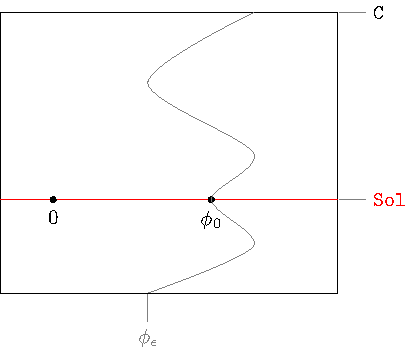
\includegraphics[width=\textwidth]{Pictures/GeometricPicture0}
		\end{minipage}
		\begin{minipage}{0.5\textwidth}
			\begin{itemize}
				\item The set $\Conf$, space of kinematic configuration, is a linear manifold.\\
					For the sake of simplicity we depict it as a plane, neglecting the complexities related to infinite-dimensional manifods.
				\item Consequently, the space of solutions $ \Sol$ is a linear submanifolds, in our picture a line, containing the section $0$.
			\end{itemize}
		\end{minipage}
		\vspace{1mm}\\
			
		We recall that the main character of the Peierls' procedure are the \emph{Lagrangian densities}, elements in $\Lag(E)$.
		Abstractly, they are maps from kinematic configuration to volume form on the spacetime. From a more practical point of view we are more interested in its twofold nature:
		\begin{itemize}
			\item As the object ruling the dynamics, through the correspondence $\Lagrangian \mapsto Q_\Lagrangian$, or, eventually, as a disturbance on the fixed unperturbed Lagrangian.
			\item As a quantity evaluable on the conformations of the system, through the correspondence  $\Lagrangian \mapsto  \mathcal{O}_\Lagrangian$.
		\end{itemize}
		
		In first instance, Peierl's procedure consider a not necessarily linear fixed Lagrangian density $\chi\in \Lag(E)$. The unique constraint is posed on the support condition of $\chi$.\\
		\vspace{1mm}		
		\begin{minipage}{0.5\textwidth}
			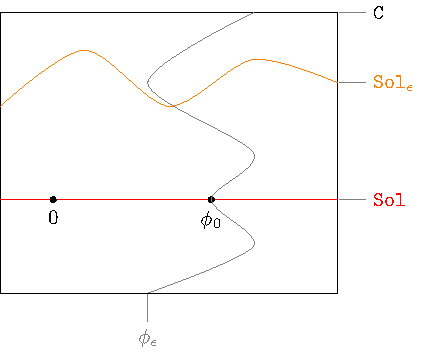
\includegraphics[width=\textwidth]{Pictures/GeometricPicture1}
		\end{minipage}
		\begin{minipage}{0.5\textwidth}
			\begin{itemize}
				\item Call $\Sol_\epsilon$ the space of solution of the disturbed dynamic equation $Q_{\Lagrangian + \epsilon \chi}$.
					Since $Q_\chi$ is generally not linear we depict this space as an arbitrary curve.\\
					Without any loss of generality we  overlook to the possibility that $\Sol \cap \Sol_\epsilon \neq \emptyset$ in this picture.
				\item To an arbitrary variation of a solution $\phi_0$ corresponds a generic parametrized curve on the plane.
			\end{itemize}
		\end{minipage}
		\vspace{1mm}
		\\
		We have proved in Section \ref{Section:PeierlsConstruction} that such choice determines two particular variation of any fixed solution $\phi_0 \in \Sol$.

		\vspace{1mm}		
		\begin{minipage}{0.5\textwidth}
			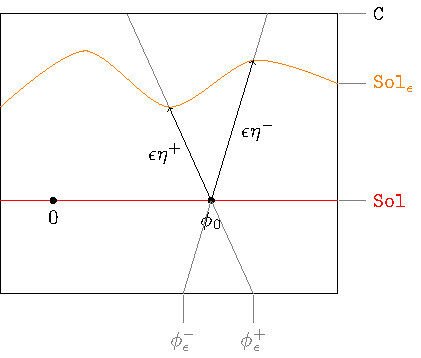
\includegraphics[width=\textwidth]{Pictures/GeometricPicture2}
		\end{minipage}
		\begin{minipage}{0.5\textwidth}
			\begin{itemize}
				\item	Among all the possible linear variations of $\phi_0$, we consider the two variation $$\phi_\epsilon^\pm = \phi_0 + \epsilon \eta_\pm$$ where $\eta_\pm$ are the unique solution of Eq. \ref{PeierlJacobiEqLin}, \textit{i.e.}:
					\begin{displaymath}
   						\eta_\pm = G^\pm \left( - Q_\chi \phi_0 \right)
					\end{displaymath}
					determined by the fixed perturbation $\chi$.
			\end{itemize}
		\end{minipage}
		\vspace{1mm}\\		
					\ifToninus \begin{Warning}
						Quando parlo di sistemi non lineari questo discorso va localizzato e linearizzato
					\end{Warning}	 \fi		
		In layman term we can say that the quantity $Q_\chi \phi_0$ quantifies how much $\phi_0$ fails to be a solution of the disturbed equations of motion.
		More explicitly :
		\begin{displaymath}
			P_\epsilon \phi_0 =  \cancel{P \phi_0} + \epsilon Q_\chi \phi_0
		\end{displaymath}
		
		The subsequent step in Peierls' procedure is the introduction of the effect operator. 
		This object can be seen as a function, associated to the disturbance $\chi$, which maps any continuous fuctional $B$ on $\Conf$ to a functional $\EffectOp_\chi^\pm B$ on $\Sol$. 

		\vspace{1mm}		
		\begin{minipage}{0.5\textwidth}
			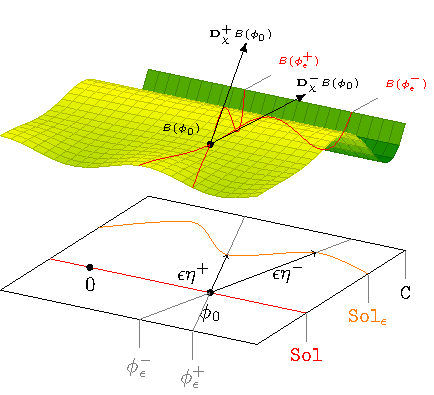
\includegraphics[width=\textwidth]{Pictures/GeometricPicture3}
		\end{minipage}
		\begin{minipage}{0.5\textwidth}
			\begin{itemize}
				\item  A generic continuous functional on the systems can be seen as a continuous function on this $\Real^2$ plane. \\ We depict them as a surface embedded in $\Real^3$.
				\item  According to that $\Sol$ can be regarded as the locus of the  \emph{"total lagrangian"} $  \mathcal{O}_\Lagrangian$ extrama.
				\item	Directly from definition \ref{EffectOperator} , we can see that $\EffectOp_\chi^\pm B$, the effect of $\chi$ on $B$ evaluated in $\phi_0$, is formally a directional derivative in the direction of $\phi_\epsilon^\pm$ calculated in point $\phi_0$.
					We depict such quantity as a tangent vector to the surface $B$ but, more properly, is corresponds to value of the inclination this vector.
			\end{itemize}
		\end{minipage}
		\vspace{1mm}\\	
		All of this machinery has a rather simpler picture when the functional $B$ is linear.

		\vspace{1mm}		
		\begin{minipage}{0.5\textwidth}
			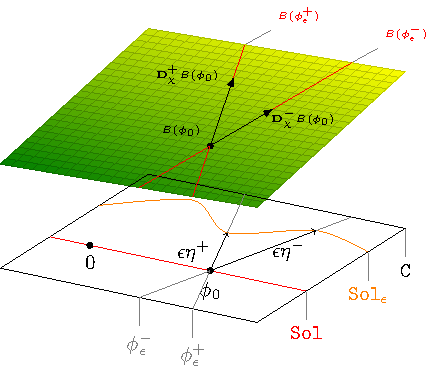
\includegraphics[width=\textwidth]{Pictures/GeometricPictureLinear1}
		\end{minipage}
		\begin{minipage}{0.5\textwidth}
			\begin{itemize}
				\item  When $B$ is a linear functional the effect takes the simple form:
					\begin{displaymath}
						\EffectOp_\chi^\pm B (\phi_0) = B ( \eta_\pm)
					\end{displaymath}
					In this case the dependence from the starting solution $\phi_0$ is accounted implicitly in the construction of perturbation $\eta_\pm(\phi_0)$.
			\end{itemize}
		\end{minipage}
		\vspace{1mm}\\	

		Finally, 
		considering two Lagrangian densities $\chi, \omega$ and the corresponding Lagrangian functional $ \mathcal{O}_\omega$, we achieve the Peierls brackets as:
		\begin{displaymath}
			\{\chi, \omega \}(\phi_0) \coloneqq \EffectOp_\chi^- \mathcal{O}_\omega (\phi_0) - \EffectOp_\chi^+ \mathcal{O}_\omega(\phi_0)
		\end{displaymath}
		According to our (\danger graphical? \danger) geometric picture we can conclude that the brackets compute the difference between the slopes of the two function $\mathcal{O}_\omega ( \phi_\epsilon^\pm)$, which can be seen as real function on the single variable $\epsilon$, calculated in $\epsilon=0$.
		We stress again that $ \phi_\epsilon^\pm$ are not arbitrary but are the specific wo variations associated to $\chi$ according to the Peierls' procedure.
		
		Thus, the brackets between $\chi$ and $\omega$ are null in three cases:
		\begin{enumerate}
			\item The two curves $\mathcal{O}_\omega ( \phi_\epsilon^+)$ and $\mathcal{O}_\omega ( \phi_\epsilon^-)$ have the same derivative when evaluated in $\phi_0$.
			\item The starting solution $\phi_0$ is also a solution of $Q_\omega$.\\
				In this case to $\phi_0$ corresponds an extremal of $\mathcal{O}_\omega$ thus its derivative is null according to each variation passing trough $\phi_0$.
			\item The starting solution $\phi_0$ is also a solution of $Q_\chi$.\\
				In this case the two perturbation $\phi_\epsilon^\pm$ are degenerate since $ \eta_\pm = 0$.
		\end{enumerate}
		
		
		\subsubsection{Peierls brackets role in second quantization.}
		The prequantum structure, in the procedure of quantization via Peierls brackets, require to restrict ourselves from the set $\Conf$ of all the global section to the space $\Gamma_0$ of compactly supported sections.

		\vspace{1mm}		
		\begin{minipage}{0.5\textwidth}
			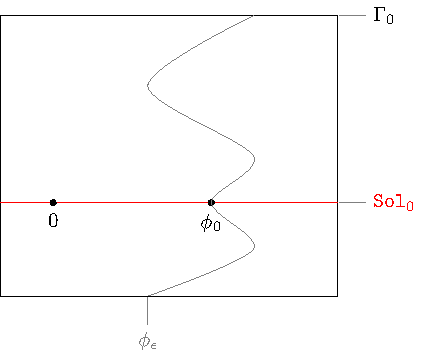
\includegraphics[width=\textwidth]{Pictures/compsupp_GeometricPicture0}
		\end{minipage}
		\begin{minipage}{0.5\textwidth}
			\begin{itemize}
				\item  For linear fields $\Gamma_0$ is still linear space, we can keep the same representation of the preceding paragraph.
			\end{itemize}
		\end{minipage}
		\vspace{1mm}\\					

	In our picture, the  choice of a pairing 
	\begin{displaymath}
		( \cdot , \cdot ) : \Gamma_0 \times \Gamma_0 \rightarrow \Real^+
	\end{displaymath}
	 ( see Section \ref{Paragraph:Pairing Construction}) correspond to the attribution of a scalar product on the plane $\Gamma_0$.
	Therefore, $\Gamma_0$ is a vector space rigged with a scalar product $(\cdot , \cdot)$.\\

	In summary, to each $f\in \Gamma_0$ we associate:
	\begin{enumerate}
		\item a continuous linear functional 
				\footnote{ One should not be misled by the extreme simplification of our geometric visualization.
				It must kept in mind that all the spaces involved are, at best, manifolds with uncountable dimensions.
				Important results as the theorem of Riesz-Fréchet can not be taken in account.}
			on $\Gamma_0$:
			\begin{displaymath}
				F_f(\cdot) = (f, \cdot)
			\end{displaymath}

		\item a Lagrangian density:
			\begin{displaymath}
				f \mapsto \Lagrangian_f \coloneqq \left\langle  f , \cdot \right\rangle_{(x)}
			\end{displaymath}
			where $<\cdot,\cdot>$ is the inner product on the configuration bundle $E$ and such that $F_f \equiv \mathcal{O}_{\Lagrangian_f}$.
		\item a Euler-Lagrange operator:
			\begin{displaymath}
				Q_{f}(\gamma) = - f \qquad \gamma \in \Conf
			\end{displaymath}
			which maps every kinematic configuration in $-f \in \Gamma_0$.
	\end{enumerate}
	In virtue of these correspondence, the Peierls' procedure allows us to equip the space $\Gamma_0$ with a pre-symplectic structure
	\begin{displaymath}
		\tau(f,g) =  \left\lbrace \Lagrangian_f , \Lagrangian_g \right\rbrace = \left( f, (\GreenAdv - \GreenRet) g \right)
	\end{displaymath}
	%
	\vspace{2mm}\\
	Let us visualize this construction in details.
	
		\vspace{1mm}		
		\begin{minipage}{0.5\textwidth}
			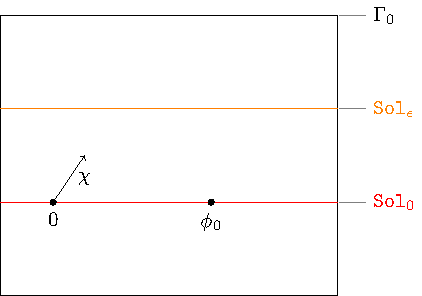
\includegraphics[width=\textwidth]{Pictures/compsupp_GeometricPicture1}
		\end{minipage}
		\begin{minipage}{0.5\textwidth}
			\begin{itemize}
				\item  We are considering only Lagrangian densities constructed from elements of $\Gamma_0$, these can be depicted as vectors on the plane $\Gamma_0$.
				\item 	$\Sol_\epsilon$ consists of all the sections $\gamma \in \Gamma_0$ such that:
					\begin{displaymath}
						P_\epsilon \gamma = ( P  - \epsilon Q_\chi) \gamma = P \gamma - \epsilon \chi = 0
					\end{displaymath}
					\textit{i.e. :} are solutions of the inhomogeneous equation $P \gamma = \epsilon \chi$.
			\end{itemize}
		\end{minipage}
		\vspace{1mm}
		
		Remembering that the solutions of a inhomogeneous differential problem can be made out superposing solutions of the homogeneous problem with a "particular solution", 
		we can affirm that
		\begin{displaymath}
			\Sol_\epsilon = \left\lbrace \phi + \epsilon G^\pm \chi \quad \vert \phi \in \Sol \quad  \right\rbrace =
			 \Sol + \epsilon \GreenAdv \chi = \Sol + \epsilon \GreenRet \chi
		\end{displaymath}
		and depict this space as a line parallel to $\Sol$.

		
		
		\vspace{1mm}		
		\begin{minipage}{0.5\textwidth}
			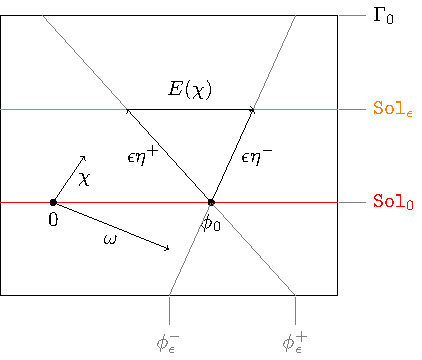
\includegraphics[width=\textwidth]{Pictures/compsupp_GeometricPicture2}
		\end{minipage}
		\begin{minipage}{0.5\textwidth}
			\begin{itemize}
				\item In this case the directions $\eta_\pm$ of the Peierls' variation $\phi_\epsilon^\pm = \phi_0 + \epsilon \eta_\pm$ of a fixed $\phi_0 \in \Sol $ are independent from $\phi_0$:
				\begin{displaymath}
					\eta_\pm = G^\pm (- Q_\chi \phi_0 ) = G^\pm \chi
				\end{displaymath}
				\item consequently $E \chi = (\GreenAdv - \GreenRet) Q_\chi \phi_0$ is always a vector on the line $\Sol_\epsilon \parallel \Sol_0$.\\
				This has been proved in Theorem:	\ref{Teo:IsomorphismBetweenTheTwoSymplectic} through the definition of the isomorphism $\Xi$.
			\end{itemize}
		\end{minipage}
		\vspace{1mm}\\		
	
		The effect of disturbance $\chi$ on an arbitrary continuous linear functional is:
		\begin{displaymath}
			\EffectOp_\chi^\pm B (\phi_0)=B (\eta_\pm) = B ( G^\pm \chi) \qquad \forall \phi_0 \in Sol
		\end{displaymath}		
		Considering instead the Lagrangian functional relative to $\omega \in \Gamma_0$ we find
		\begin{displaymath}
			\EffectOp_\chi^\pm F_\omega (\phi_0) = \left( \omega , G^\pm \chi \right)
		\end{displaymath}
		which leads to the pre-symplectic form $\tau$.
		
				\vspace{1mm}		
		\begin{minipage}{0.5\textwidth}
			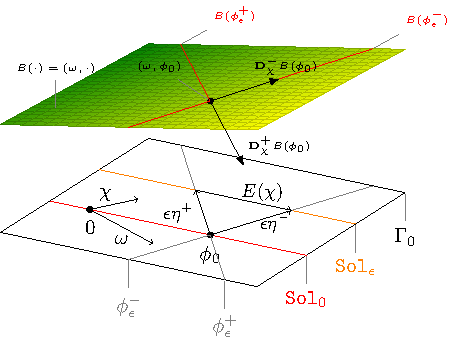
\includegraphics[width=\textwidth]{Pictures/compsupp_GeometricPictureLinear}
		\end{minipage}
		\begin{minipage}{0.5\textwidth}
			\begin{itemize}
				\item For the sake of simplicity we depict the pairing relation as the ordinary inner product  on the plane $\Gamma_0$.
				\item The Lagrangian functional $B_\omega (\cdot) = (\omega, \cdot)$ correspondent to  $\omega \in \Gamma_0$  can be depicted as a plane which intersect plane $ x y$ along the normal to $\omega$.
			\end{itemize}
		\end{minipage}
		\vspace{1mm}\\	
	
		In conclusion, according to our visualization, the brackets between $\chi$ and $\omega$ are null when:
		\begin{displaymath}
		 \omega \perp E \chi \Longleftrightarrow \chi \perp E \omega
		\end{displaymath}
		where the perpendicularity condition is intended in respect to the inner product on $\Gamma_0$ induced by pairing.
		
		\begin{Warning}
			Osservando la figura si potrebbe dedurre che 
			\begin{displaymath}
				\omega \perp \Sol_0 \quad \Rightarrow \qquad \{\omega, \chi\} = ( \omega , E \chi)=0 \qquad \forall \chi \in \Gamma_0
			\end{displaymath}
			Ma io ho anche detto che :
			\begin{displaymath}
				E \chi \parallel \Sol_0 \qquad \forall \chi \in \Gamma_0
			\end{displaymath}
			Quindi ho un assurdo
			\begin{displaymath}
				 0 = ( \omega , E \chi)=-( E\omega ,  \chi)\neq 0
			\end{displaymath}
			?\\
			No, se posso provare che 
			\begin{displaymath}
				(\omega, \phi) = 0 \quad \forall \phi \in \Sol_0  \qquad \Rightarrow  \quad(\GreenAdv - \GreenRet) Q_\omega \phi_0= 0 
			\end{displaymath}
			Questo è ragionevole perchè il funzionale $\mathcal{O}_\omega (\cdot) = ( \omega, \cdot): \Conf \rightarrow \Real$ se ridotto di domino a $\Sol$ è identicamente nullo ( $\ker(\mathcal{O}_\omega) \supset \Sol$) e  dovrebbe dare $\left. Q_\omega \right\vert_\Sol = 0$.
			\\ non sono sicuro che si possa fare così... 
			
			
		\end{Warning}
	
		\subsubsection{Peierls Brackets of the Jacobi field}
		Now we take a step further considering the Peierls brackets in the case of a Jacobi Fields.
		\begin{figure}[h!]
			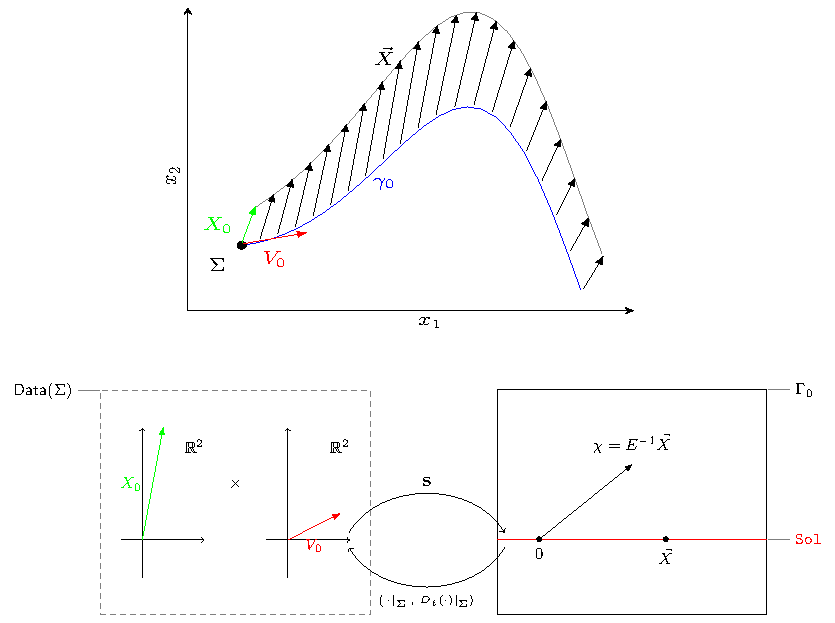
\includegraphics[width=\textwidth]{Pictures/Jacobi_GeometricPicturePanoramica}	
			\caption{ 
			%Impressionistic representation of the Jacobi field system on a  2-dimensional Riemannian manifold $M$.\\
			Below: the geometric structures encoding the "pre-quantum" Jacobi field.
			\\
			Above: a local chart representation of a Jacobi field $\vec{X}$ along a fixed geodesic $\gamma_0$ on a  2-dimensional Riemannian manifold $M$.
			}	
		\end{figure}				

		This example provides a testing ground on which compare the two pre-quantization procedures showed in Chapter 3.\\
		The crucial point is that the following correspondences:
		\begin{displaymath}
			(\chi) \in \Gamma_0 \quad \xmapsto{\Xi} \quad (E \chi) \in \Sol \quad \xmapsto{\vert_\Sigma} \quad 
			 \left(\left. E\chi \right\vert_\Sigma , D_t\left.\left( E \chi \right)\right\vert_\Sigma \right) \in\Data(\Sigma)
		\end{displaymath}
		\begin{displaymath}
			 \left(\substack{a\\b}\right) \in\Data(\Sigma) \quad \xmapsto{\SolMap} \quad
			 \left( \SolMap \left(\substack{a\\b}\right) \right)\in \Sol \quad \xmapsto{E^{-1}} \quad 
			 \left( E^{-1}\SolMap \left(\substack{a\\b}\right) \right) \in \Gamma_0
		\end{displaymath}
		are symplecto-morphism. This allows us to compare the symplectic form $\tau$ on $\Obs$ with the symplectic form $\Omega$ on $\Data(\Sigma)$.
		
		\vspace{1mm}
		In order to obtain a more intuitive representation we limit ourselves to the most simple case of one-dimensional Riemannian manifolds.

	\subsection{Geometric Mechanics of Classical Fields}
	
	L'idea è che tutta l'immagine precedente richiederebbe una further investigation from a mathematica point of view per essere ammessa come rigorosa.
	The covariant phase space of a system in physics is the space of all of its solutions to its classical equations of motion, the space of classical trajectories of the system. 
 Typically these phase spaces are (locally) naturally parameterized by the suitable boundary conditions or choice of a Cauchy surface which uniquely determine the corresponding history of the physical system. This parameterization is what traditionally is just called a “phase space”. 
	The “covariant” in “covariant phase space” is to indicated that it comes without any unnatural choices.
	
 For instance for a non-relativistic particle propagating on a Riemannian manifold $X$ with the usual action functional, a trajectory is uniquely fixed by the position $xi \in X$ and the momentum $p\in T^*_x X$ of the particle at a given time. 
 Correspondingly the space of all solutions and hence the (covariant) phase space of the system may be identified with the cotangent bundle $T^*X$ of $X$.

 The covariant phase space can be embedded into the space of field configurations as a subspace of the set of solutions that transversely intersects gauge orbits.  
 This embedding is characterized as the zero locus of the equations of motion and some gauge fixing conditions. The non-degenerate Poisson structure on the algebra of functions on the covariant phase space is given by the Peierls bracket.

 The Peierls bracket of two functions $A$ and $B$ is the antisymmetrized influence on $B$ of an infinitesimal perturbation of a gauge-fixed action by function that restricts to A on the embedding. 
 The algebra of functions on the space of field configurations becomes a Poisson algebra in the following way. Pick a set of functions on the space of field configurations that restrict to a non-degenerate coordinate system on the embedded covariant phase space. 
 These functions, together with the equations of motion and gauge fixing conditions define a Poisson bivector by being declared canonical, such that the kernel of the bivector coincides with the ideal generated by the equations of motion and the gauge fixing conditions. 
 Obviously the Poisson structure thus constructed on the algebra of functions on field configurations is not unique and depends on the above choice of coordinates; the same non-uniqueness may be parametrized instead by a choice of a connection on the space of field configurations. 
 The embedded covariant phase space becomes a leaf of the symplectic foliation of the space of field configurations.

 However, even reduced phase spaces are not all cotangent bundles, typically not, for instance, if they are obtained by symplectic reduction. 
 This way a finite-dimensional phase space can sometimes describe continuous systems (e.g. in hydrodynamics) whch have infinitely many degrees of freedom; that phase space is however not a cotangent bundle of something in general.

 \begin{example}
  The covariant phase space of the relativistic particle on a pseudo-Riemannian manifold X is the space of geodesics of X (in the absence of a background gauge field).
 \end{example}






\end{document}

